\chapter{Results and Discussion}

\section{Overview}

Table~\ref{tab:summary} shows the average RPD and total computation time for
all 14 algorithm configurations, sorted from best to worst solution quality.

\begin{table}[H]
\centering
\caption{Average RPD (\%) and total computation time (seconds) across all 78
instances. FI = first-improvement, BI = best-improvement;
Tra/Exc/Ins = transpose, exchange, insert; Rnd = random init, CW =
Chenery-Watanabe.}
\label{tab:summary}
\small
\begin{tabular}{llllrr}
\toprule
Algorithm & Pivot & Neighbourhood & Init & Avg RPD (\%) & Total time (s) \\
\midrule
VND2 & FI & Tra$\to$Ins$\to$Exc & CW & 1.92 & 136.1 \\
VND1 & FI & Tra$\to$Exc$\to$Ins & CW & 2.02 & 205.7 \\
II   & FI & Insert              & CW  & 2.02 & 138.8 \\
II   & FI & Insert              & Rnd & 2.02 & 204.2 \\
II   & BI & Insert              & CW  & 2.26 & 35.9 \\
II   & BI & Insert              & Rnd & 2.30 & 40.2 \\
II   & FI & Exchange            & Rnd & 2.82 & 228.0 \\
II   & FI & Exchange            & CW  & 2.97 & 189.6 \\
II   & BI & Exchange            & Rnd & 3.60 & 35.6 \\
II   & BI & Exchange            & CW  & 3.85 & 32.5 \\
II   & BI & Transpose           & CW  & 17.08 & 0.23 \\
II   & FI & Transpose           & CW  & 17.09 & 0.21 \\
II   & BI & Transpose           & Rnd & 34.47 & 0.002 \\
II   & FI & Transpose           & Rnd & 34.61 & 0.002 \\
\bottomrule
\end{tabular}
\end{table}

Looking at the table, the neighbourhood choice is clearly the biggest factor.
Insert-based algorithms all land around 2--2.3\% RPD, exchange around
2.8--3.9\%, and transpose is far behind at 17--35\%. Figure~\ref{fig:barplot_full}
makes this separation very visible.

\begin{figure}[H]
    \centering
    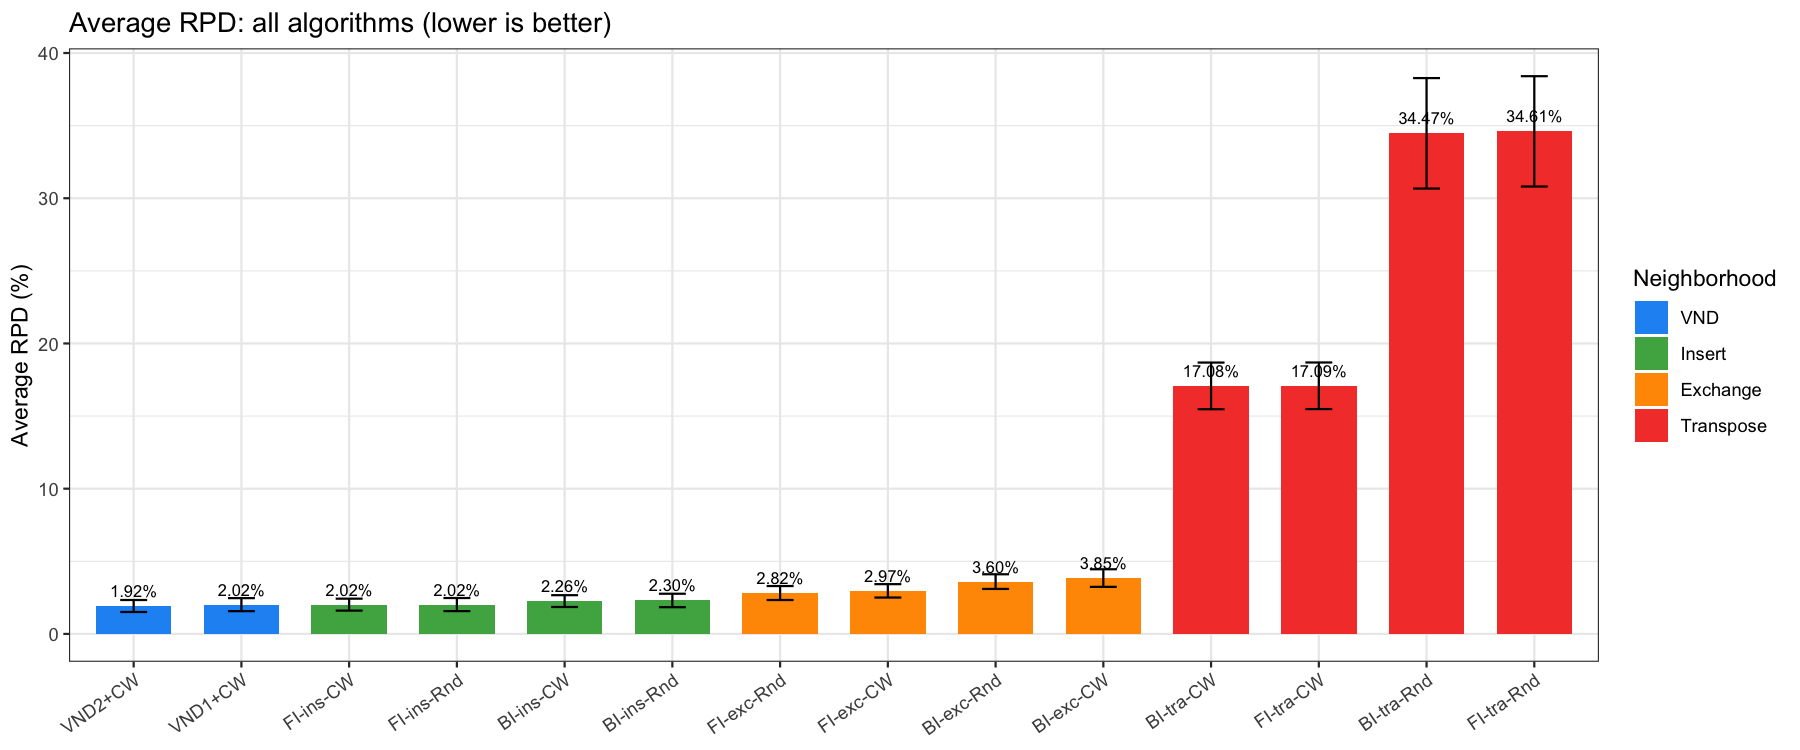
\includegraphics[width=\linewidth]{figures/barplot_avg_rpd_full.png}
    \caption{Average RPD (\%) for all 14 configurations. Error bars show 95\%
    confidence intervals. The colour groups (red = Transpose, orange =
    Exchange, green = Insert, blue = VND) show how much the neighbourhood
    structure drives the final quality.}
    \label{fig:barplot_full}
\end{figure}

The transpose neighbourhood performs so poorly because it only considers
$n - 1$ adjacent swaps at each step. On instances of size 150 or 250, that is
far too few moves to make any real progress, especially from a random starting
point. Exchange and insert both consider $O(n^2)$ moves and have much more
freedom to improve the solution.

Figure~\ref{fig:boxplot} shows the full RPD distributions. The insert and VND
algorithms are not only better on average but also more consistent across
instances. Transpose has a very wide spread, which means it is sensitive to
which particular instance it runs on.

\begin{figure}[H]
    \centering
    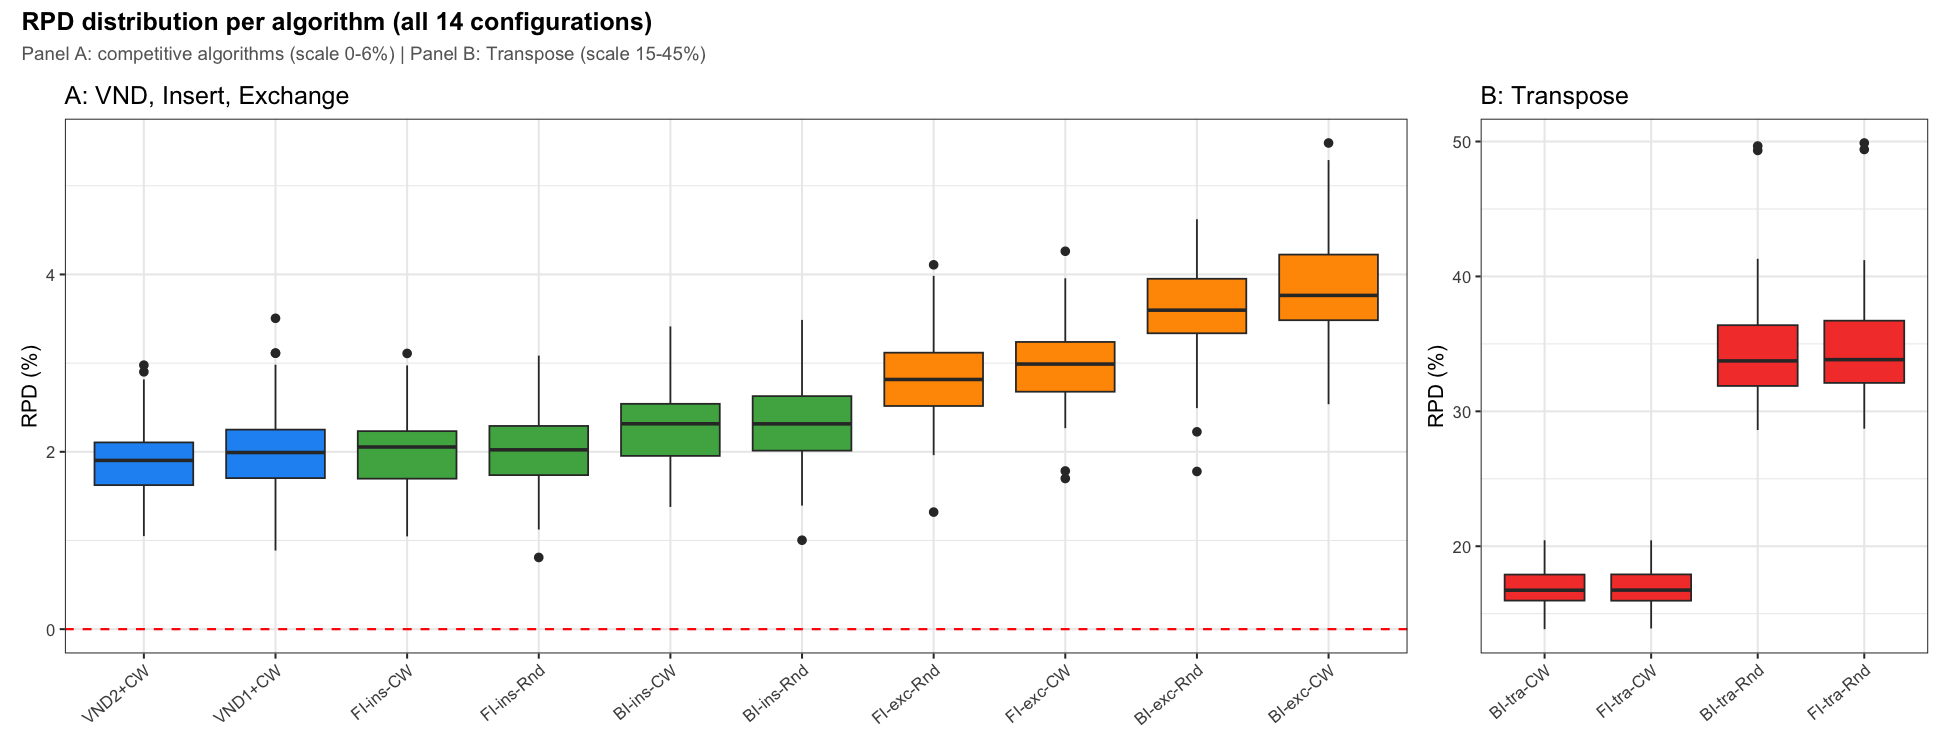
\includegraphics[width=\linewidth]{figures/boxplot_rpd_full.png}
    \caption{RPD distribution across the 78 instances. Panel A shows the
    competitive algorithms (scale 0--6\%); Panel B shows transpose on a
    larger scale (15--45\%) to make the spread visible.}
    \label{fig:boxplot}
\end{figure}

\section{Exercise 1.1 --- Iterative Improvement}

\subsection{Pivoting rule}

For insert, first-improvement (2.02\%) consistently beats best-improvement
(2.26--2.30\%), and this difference is statistically significant ($p < 0.001$
in all cases). At first this is a bit surprising --- you would expect that
always picking the best available move leads to a better solution. But what
seems to happen is that best-improvement takes fewer, larger steps and gets
stuck in local optima that first-improvement avoids by moving more quickly
through the search space. A similar pattern holds for exchange.

For transpose, the pivoting rule barely matters once the CW heuristic is used
($p = 0.097$). With only $n-1$ neighbours to explore, both rules behave
almost identically.

\subsection{Neighbourhood structure}

All pairwise comparisons between neighbourhood types are highly significant
($p < 0.001$): insert beats exchange, and exchange beats transpose, without
exception. Figure~\ref{fig:barplot_zoom} zooms in on the competitive
algorithms to make the insert/exchange gap clearer.

\begin{figure}[H]
    \centering
    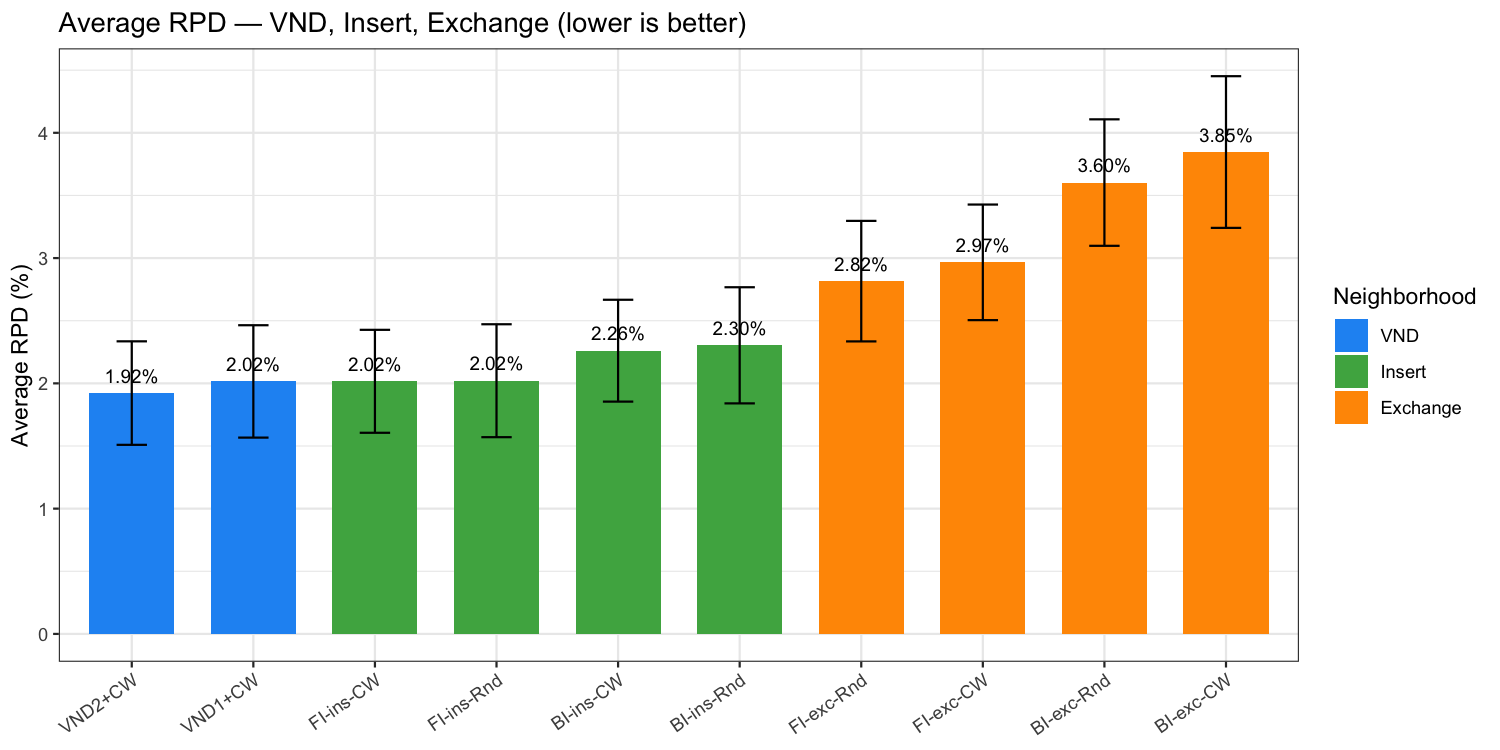
\includegraphics[width=\linewidth]{figures/barplot_avg_rpd_zoom.png}
    \caption{Average RPD for VND, Insert, and Exchange configurations only
    (transpose excluded for scale). First-improvement is better than
    best-improvement in both insert and exchange.}
    \label{fig:barplot_zoom}
\end{figure}

\subsection{Initialisation}

The effect of initialisation depends a lot on the neighbourhood. For
transpose, switching from random to CW cuts the RPD from $\sim$34\% down to
$\sim$17\% --- a massive improvement that is clearly significant ($p <
0.001$). For exchange, CW also helps ($p = 0.014$ for FI, $p = 0.002$ for
BI). But for insert, initialisation makes essentially no difference: $p =
0.909$ for FI-insert and $p = 0.557$ for BI-insert. The insert neighbourhood
is large enough to fix a bad starting point on its own, so there is not much
point in using CW when insert is the chosen neighbourhood.

\subsection{Statistical overview}

Figure~\ref{fig:heatmap} shows the Wilcoxon $p$-values for all pairwise
comparisons. Almost everything is red (significant), which confirms that most
algorithm configurations are genuinely different from one another. The few
green cells appear mainly between the best-performing algorithms, where the
differences are small.

\begin{figure}[H]
    \centering
    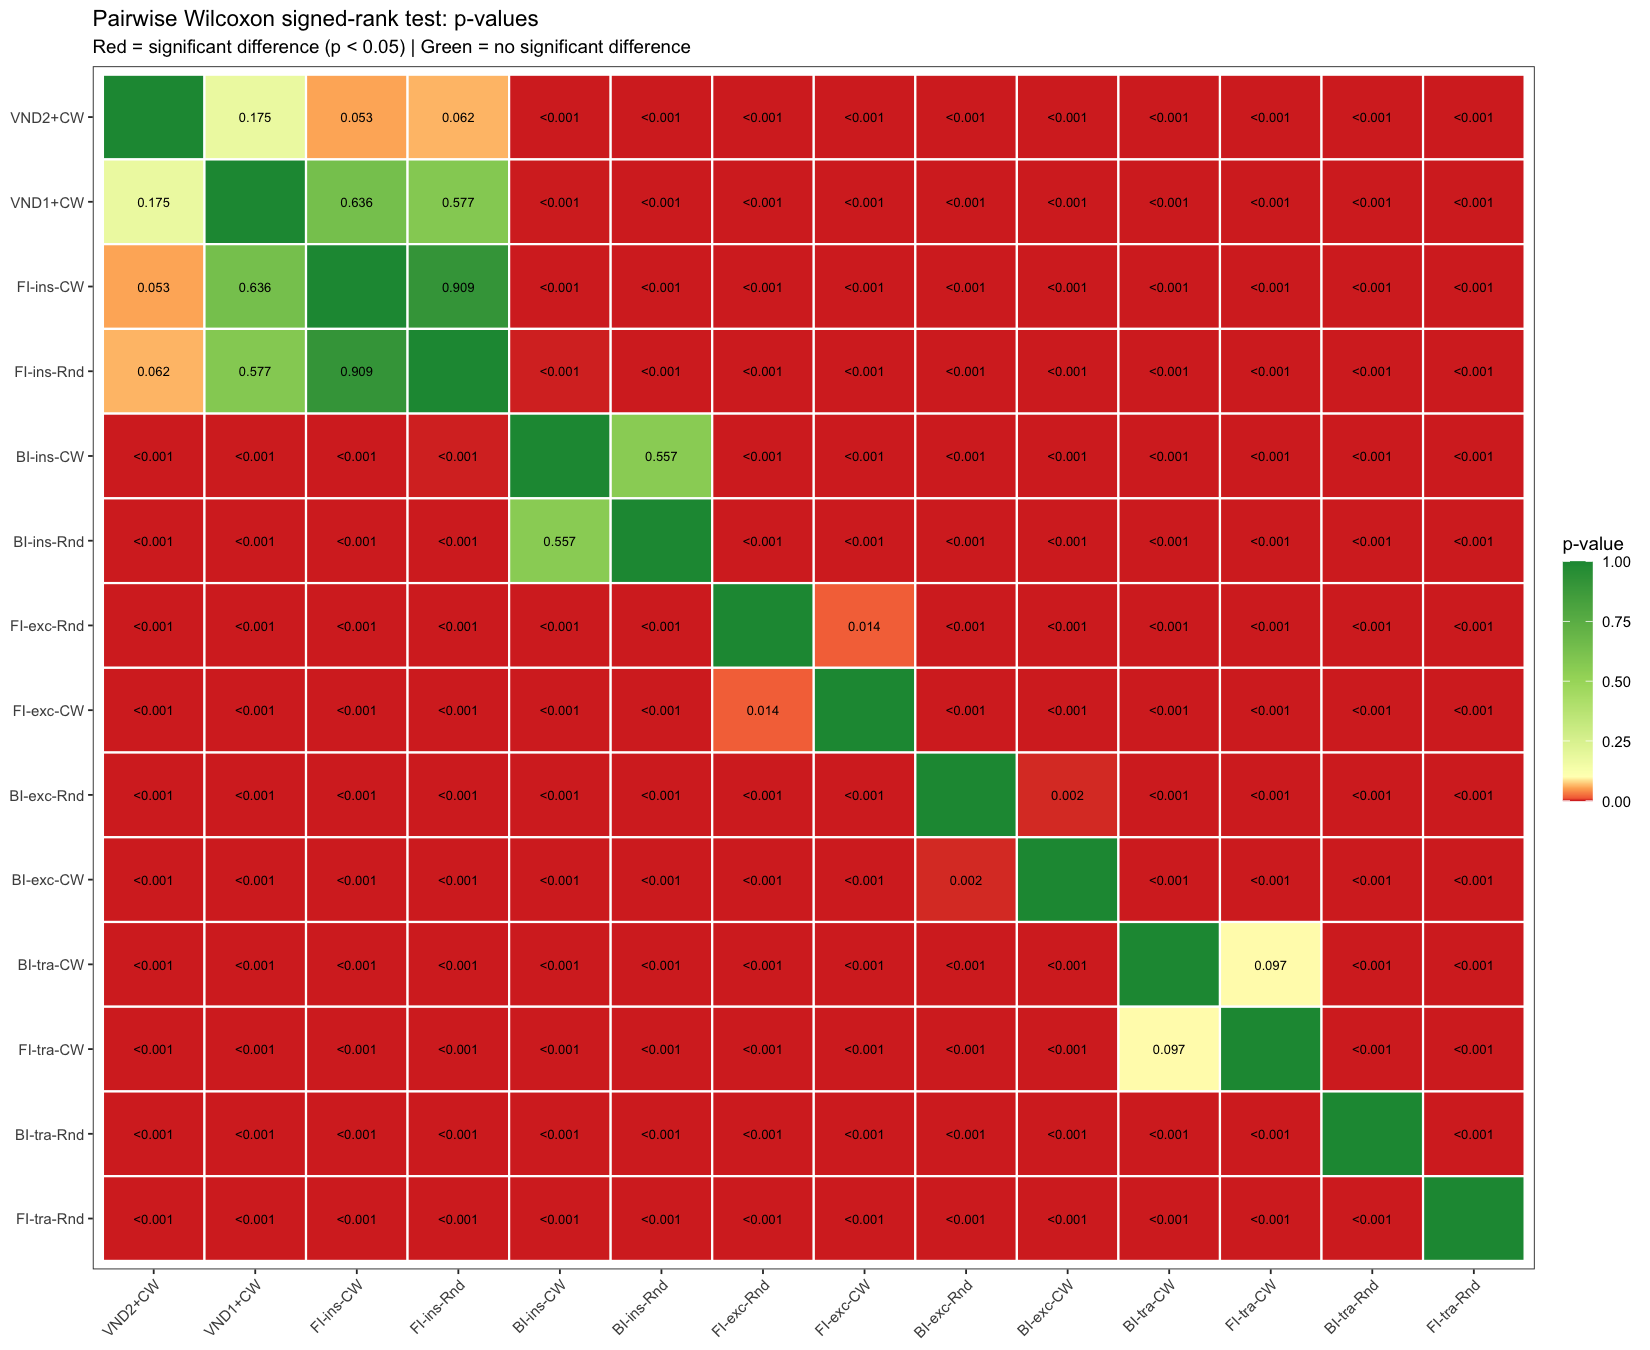
\includegraphics[width=\linewidth]{figures/heatmap_pvalues.png}
    \caption{Pairwise Wilcoxon signed-rank $p$-values. Red = significant
    ($p < 0.05$), green = not significant. Most pairs differ significantly;
    the exceptions are among the top-ranked algorithms.}
    \label{fig:heatmap}
\end{figure}

\section{Exercise 1.2 --- Variable Neighbourhood Descent}

\subsection{VND1 vs VND2}

VND2 (Tra $\to$ Ins $\to$ Exc) achieves 1.92\% RPD and VND1 (Tra $\to$ Exc
$\to$ Ins) achieves 2.02\%. The difference is not statistically significant
($p = 0.176$), so we cannot conclude that one ordering is better than the
other. In practice, both orderings benefit from the same idea: start with the
cheapest neighbourhood (transpose) to pick up easy gains, then switch to the
heavier ones to refine the solution.

\subsection{VND vs single-neighbourhood}

Comparing VND to the best single-neighbourhood algorithm (FI-insert-CW, also
at 2.02\% RPD), the differences are again not significant: $p = 0.636$ for
VND1 and $p = 0.053$ for VND2. So adding two extra neighbourhoods on top of
insert does not reliably improve the final result on these instances. The
insert neighbourhood is already strong enough on its own.

\subsection{Quality vs. computation time}

Figure~\ref{fig:qvst} plots average RPD against total computation time. The
trade-off is interesting: best-improvement algorithms (for insert and exchange)
run much faster but reach worse solutions. First-improvement insert and both
VND variants sit in a good spot --- competitive quality at moderate cost.
Transpose is in a category of its own: extremely fast but nowhere near useful.

\begin{figure}[H]
    \centering
    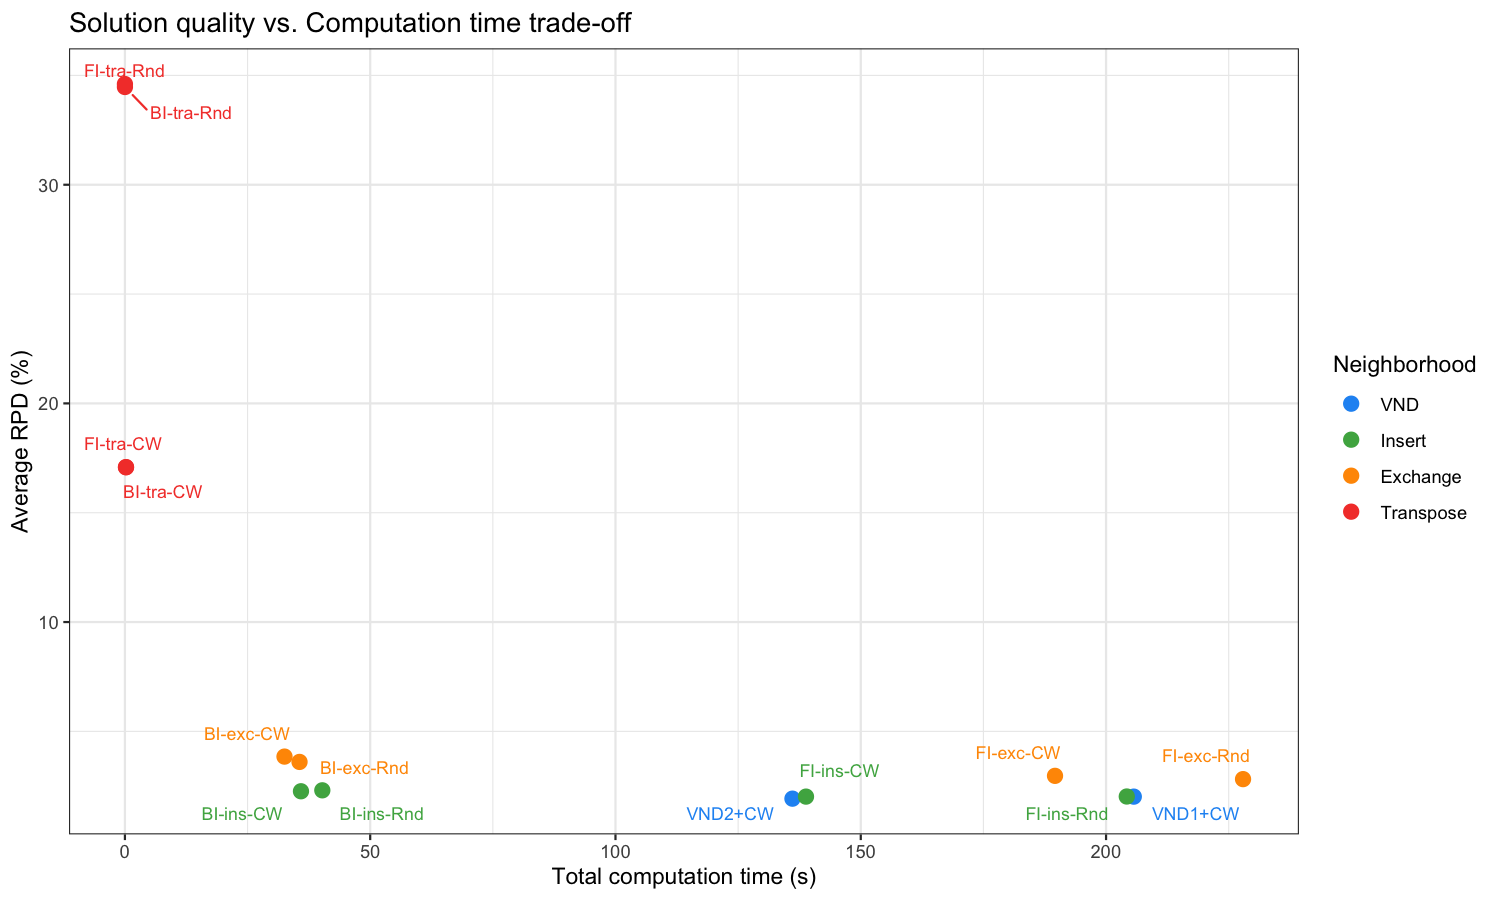
\includegraphics[width=0.85\linewidth]{figures/rpd_vs_time.png}
    \caption{Average RPD vs total computation time across all 78 instances.
    Insert FI and VND offer the best quality-to-time trade-off. Transpose is
    fast but ineffective. Best-improvement runs faster but finds worse local
    optima than first-improvement.}
    \label{fig:qvst}
\end{figure}

VND2 is also faster than VND1 (136 s vs 206 s total) while achieving slightly
better quality, which suggests that visiting insert before exchange is more
efficient --- insert likely resolves most of the remaining improvements,
leaving less work for exchange to do.
